%%%%%%%%%%%%%%%%%%%%%%%%%%%%%%%%%%%%%%%%%
%
% (c) 2021 by Jennifer Laaser
%
% This work is licensed under the Creative Commons Attribution-NonCommercial-ShareAlike 4.0 International License. To view a copy of this license, visit http://creativecommons.org/licenses/by-nc-sa/4.0/ or send a letter to Creative Commons, PO Box 1866, Mountain View, CA 94042, USA.
%
% The current source for these materials is accessible on Github: https://github.com/jlaaser/pogil-polymers
%
%%%%%%%%%%%%%%%%%%%%%%%%%%%%%%%%%%%%%%%%%

\renewcommand{\figpath}{content/polymchem/livingpolyms/ATRP/figs}
\renewcommand{\labelbase}{ATRP}

\begin{activity}{Atom Transfer Radical Polymerization}

\begin{instructornotes}
	This activity introduces students to concepts related to controlled radical polymerization via Atom Transfer Radical Polymerization (ATRP)
	
	After completing this activity, students will be able to:
	\begin{enumerate}
		\item ...
	\end{enumerate}
	
	\subsection*{Activity summary:}
	\begin{itemize}
		\item \textbf{Activity type:} Learning Cycle
		\item \textbf{Content goals:} Thermodynamics of free-radical polymerization
		\item \textbf{Process goals:} %https://pogil.org/uploads/attachments/cj54b5yts006cklx4hh758htf-process-skills-official-pogil-list-2015-original.pdf
			written communication, critical thinking, information processing
		\item \textbf{Duration:} TBD
		\item \textbf{Instructor preparation required:} none beyond knowledge of relevant content
		\item \textbf{Related textbook chapters:}
			\begin{itemize}
				\item \emph{Polymer Chemistry} (Hiemenz \& Lodge): section NNN
			\end{itemize}
		%\item \textbf{Facilitation notes:}
		%	\begin{itemize}
		%		\item \dots
		%	\end{itemize}
	\end{itemize}
	
\end{instructornotes}


\begin{model}[Key Reactions in ATRP]
	\label{\labelbase:mdl:ATRPrxns}

	Atom Transfer Radical Polymerization (ATRP) is a popular method for obtaining narrow molecular weight distributions in radical polymerizations.  The key reactions involved in ATRP are:
	
	\centerline{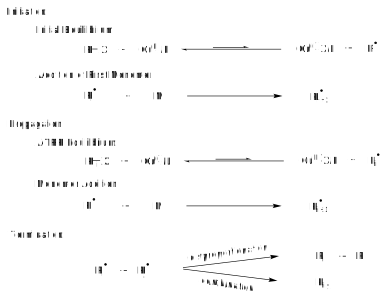
\includegraphics[width=0.8\textwidth]{\figpath/Model1_scheme}}
	
	Here, ``RX'' is an alkyl halide initiator, ``Cu\textsuperscript{(I)}/L'' is a copper-based catalyst, ``M'' is the monomer, and the ``P$_i^\bullet$'' are the propagating chains of length $i$.
	
\end{model}


\begin{ctqs}

	\question Achieving a truly ``living'' polymerization requires there to be no irreversible termination reactions.
	
		\begin{enumerate}
		
			\item Is this criterion strictly obeyed for the reaction scheme shown in Model \ref{\labelbase:mdl:ATRPrxns}?  Why or why not?  \label{\labelbase:ctq:terminationsuprression}
			
				\begin{solution}[1in]
				\end{solution}
			
			\item Recall that in radical polymerizations, the termination rate is given by
				\begin{equation*}\
					R_t = 2k_t[\text{P}^\bullet]^2
				\end{equation*}
				What needs to be true about the concentration of active radicals, [P$_i^\bullet$], to keep this termination rate as low as possible?
				
				\begin{solution}[1in]
				\end{solution}
			
		\end{enumerate}
	
	\question The key equilibrium that determines the active radical concentration is the ATRP equilibrium,
	
	\centerline{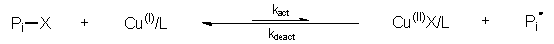
\includegraphics[width=0.7\textwidth]{\figpath/Model1_KATRP}}
		
		\begin{enumerate}
			\item Based on your answer to the previous question, does achieving good control over the molecular weight of polymers synthesized by ATRP require this reaction to favor the left side or the right side of the reaction?
			
				\begin{solution}[1in]
				\end{solution}
			
			\item What must be true about the value of $K_{ATRP}$ if you want to control the molecular weight of polymers synthesized by ATRP?
			
				\begin{solution}[1in]
				\end{solution}
			
		\end{enumerate}

\end{ctqs}

\begin{infobox}
	The structures of several popular ligands used to make catalysts for ATRP, and their equilibrium constants, are:
	
	\centerline{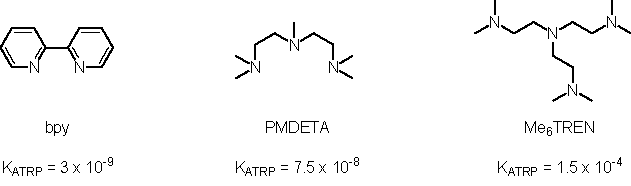
\includegraphics[width=0.8\textwidth]{\figpath/ATRP_ligands}}
\end{infobox}

\begin{ctqs}
	
	\question Which ligand would you expect to give the best dispersity in an ATRP reaction?  Briefly explain your group's reasoning in 1-2 complete sentences.
	
		\begin{solution}[1.25in]
		\end{solution}
	
	\question If you use a ligand that has \emph{too high} of a value of $K_{ATRP}$, what do you expect to happen to the dispersity of the polymer chains?  Suggest one change you could make to the reaction conditions to mitigate this problem.
	
		\begin{solution}[1.25in]
		\end{solution}
	
	\question If you use a ligand that has \emph{too low} of a value of $K_{ATRP}$, what do you expect to happen to the overall polymerization rate?  Suggest one change that you could make to the reaction conditions to mitigate this problem.
	
		\begin{solution}[1.25in]
		\end{solution}
	
	\question All of the ligands shown above contain nitrogen centers that coordinate to the Cu\textsuperscript{(I)} species to form the active catalyst.
	
		Why might monomers containing primary, secondary, or tertiary amines in their sidechains be difficult to polymerize by ATRP?  
	
		\begin{solution}[1.25in]
		\end{solution}
	
\end{ctqs}

\begin{infobox}
	One popular initiator for ATRP is ethyl 2-bromoisobutyrate, or EBriB.  Its structure is shown below:
	
	\centerline{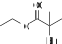
\includegraphics[width=0.2\textwidth]{\figpath/EBriB}}
\end{infobox}

\begin{ctqs}
	\question Draw the structure of the active radical R$^\bullet$ that you expect to be formed when this intiator is activated by the copper catalyst (\emph{hint: remember that the ``X'' in ``RX'' is a stand-in for a halogen atom}):
	
		\begin{solution}[1.5in]
		\end{solution}
	
	\question Draw the structure that would be formed if this radical attacks a methyl methacrylate monomer (that is, draw RM$^\bullet$, where the monomer M is methyl methacrylate).
	
		\begin{solution}[1.5in]
		\end{solution}
	
	\question Compare the types of radicals you drew in both of the preceding questions.
	
		\begin{enumerate}
			\item Do you expect EBriB to be a a ``good'' initiator for methacrylate monomers?  Why or why not?  Explain your group's reasoning in 2-3 complete sentences.
	
			\begin{solution}[1.25in]
			\end{solution}
			
			\item Based on your response to the previous question, propose a strategy that you could use to choose an initiator based on the structure of the monomer you want to polymerize.
	
			\begin{solution}[2in]
			\end{solution}
			
		\end{enumerate}
		
		% NOTE TO SELF: Ideally, I'd really like to get at the issue of the initial vs. ATRP equilibria and which one  needs to have a higher equilibrium constant.  Maybe also look at equilibrium constants for some of the initiators, and get at the difference between Br and Cl
		
		% I'd also like to have a question that gets at the fact that ATRP maintains high chain-end functionality - this is really critical for e.g. synthesis of block copolymers
		
		% these could go in the exercises?  Or, I could have an extension that delves more deeply into ATRP?
		
\end{ctqs}


\begin{exercises}

	\exercise ATRP is often referred to as a ``living radical polymerization''.  Is this term strictly accurate?  Why or why not?  Based on your answer, why do you think some polymer scientists prefer to call ATRP a \emph{controlled} radical polymerization rather than a living radical polymerization?
	
		\emph{Hint: you might want to revisit your answer to CTQ \ref{\labelbase:ctq:terminationsuprression}.}
		
	\exercise 
	
		\begin{enumerate}
	
			\item Which species (initiator, catalyst, or monomer) determines the number of polymer chains formed in an ATRP reaction?
	
			\item Suppose you run an ATRP reaction using 0.1~mol methyl methacrylate, 1~mmol EBriB, 1~mmol CuBr, and 2~mmol PMDETA, and you stop the reaction when it reaches 60\% conversion (i.e. when 60\% of the monomers have been incorporated into polymer chains).  What should you expect the molecular weight of the resulting polymer to be?
			
		\end{enumerate}
		
%	\exercise Although this activity primarily discussed ATRP in terms of the activation/deactivation equilibrium, kinetics matter as well.
	
%		\begin{enumerate}
%			\item Suppose a polymer chain is activated, forming a propagating radical P$^\bullet$.  If this propagating radical stays active for a ``long'' time, many new monomers will be able to add to the chain before it is deactivated, while the length of the dormant chains will not change.
			
%				Explain, in 2-3 sentences, how you expect a ``long'' radical lifetime to affect the dispersity of the polymer sample.
				
%			\item Which rate constant determines the length of time for which a radical will stay active before being deactivated?  Based on your answer to part (a), do you expect a higher or lower value of this rate constant to give a better dispersity?
			
%			\item The equilibrium constant for the ATRP equilibrium can be written
%				\begin{equation*}
%					K_{ATRP} = \frac{[\text{Cu}^{(II)}X/L][\text{P}^\bullet]}{[\text{Cu}^{(I)}X/L][\text{PX}]}
%				\end{equation*}
				
%				Use this information, and appropriate information from Activity \ref{FRPkinetics}, to write an equation for the overall polymerization rate $R_p$ in terms of $K_{ATRP}$, $k_p$, and the concentrations of any relevant chemical species.
				
%			\item The equilibrium constant for the ATRP equilibrium can \emph{also} be written as the ratio of the rate constants,
%				\begin{equation*}
%					K_{ATRP} = \frac{k_{act}}{k_{deact}}
%				\end{equation*}
%				Substitute this expression into your answer to the previous question to obtain an expression for $R_p$ in terms of $k_{act}$ and $k_{deact}$.
%				
%			\item Using your answers to the previous parts of this question, critique or defend the following statement in 2-3 complete sentences:
			
%				``In ATRP, there is usually a tradeoff between choosing a catalyst that gives a fast enough polymerization to make a useful amount of polymer, and choosing a catalyst that gives good control over the molecular weight distribution.''
%		\end{enumerate}
	
\end{exercises}


%\begin{problems}
%
%	\problem First exercise
%	\problem Second exercise
%	
%\end{problems}


	
\end{activity}